\section{Chat Room}
Der er i projektet blevet lavet et Chat Room, der er udviklet med SignalR packagen fra NuGet. Dette afsnit beskriver hvordan den del af sitet er designet og implementeret. Der i taget udgangspunkt i Microsofts SignalR eksempel.  \cite{SignalR}

\subsection{Chat Controller}
Chat controlleren bruger en unit of work til at videregive brugerens navn til chatten, så brugernes navn vil fremgå når brugeren skriver beskeder i chat roomet. 
 
\subsection{Chat Hub}
Chat hubben er den pipeline der kommer til at være imellem client og server. Denne forbindelse gør at SignalR kan kalde tilbage til serveren, med kald direkte i mellem de to. Oprettelsen af denne forbindelse sikrer at brugeren vil opleve ændringerne i real time, da der ikke findes kø ned til serveren. 
Hubben har desuden funktionen: 
\begin{lstlisting}
Clients.All.addNewMessageToPage(name, message);
\end{lstlisting}
som kalder ned i SignalR pakken. Herefter sørger SignalR for at få denne besked broadcastet til alle clients, i realtime, som sidder på siden. 

\subsection{Sekvens diagram af Chat room}
\begin{figure}[H]
	\centering
	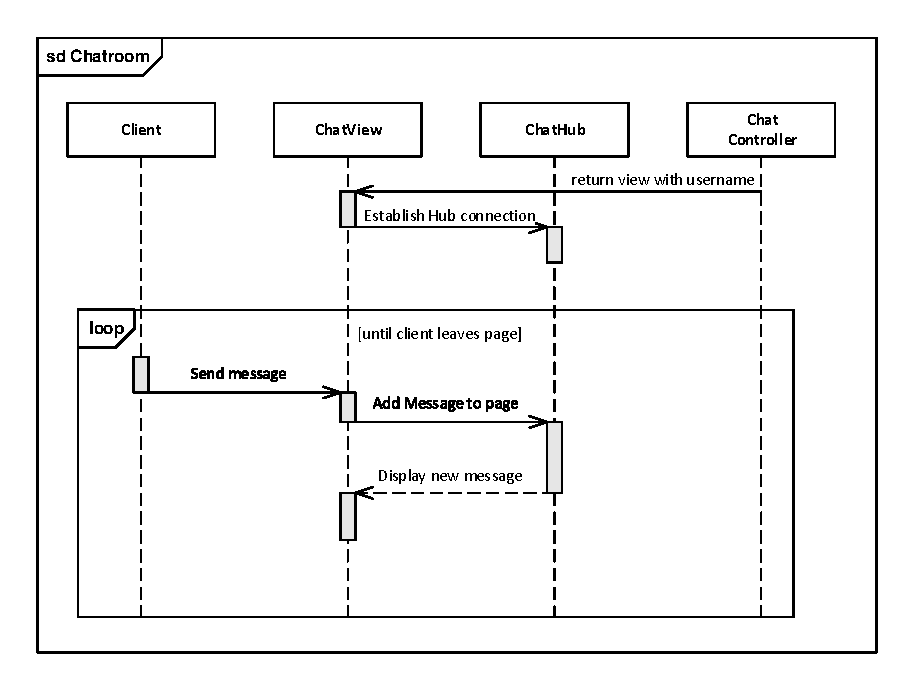
\includegraphics
	[width=165mm]{figures/signalrdiagram.pdf}
	\caption{Sekvens diagram for forløbet af chat afviklingen. }
	\label{fig:signalrdiagram}
\end{figure}

Diagrammet på figur \ref{fig:signalrdiagram} viser forløbet når brugeren tilgår chatroomet. Brugerens navn bliver sendt med videre til viewet igennem controlleren gennem Unit of Work, og viewet kan nu bruge navnet i forbindelse med udskrivning af beskeder. Viewet ude ved brugeren opretter derefter en hub connection tilbage til serveren. Brugeren har nu mulighed for at skrive beskeder i chatroomet, så længe han fortsat er på siden. 

\subsection{Chat view}
Eftersom det hele skal forgå realtime, bliver der i viewet anvendt javascript for at give brugeren den nødvendige interaktion. Signalr autogenerer et par mapper som holder den nødvendige infomation i den tid brugeren er på dette view. 
Viewet binder som det første funktionen fra Hub klassen til den liste, der er container for chat beskederne. Næste punkt er at starte forbindelsen mellem client og server. 

\begin{lstlisting}
 $.connection.hub.start().done(function () {
if (firsthit === 0) {
chat.server.send($('#displayname').val(), "har joinet chatten!");
firsthit++;
}
\end{lstlisting}

På kodeeksemplet kan vi se at når vi har fået forbindelse til serveren, og dette er gået godt, skrives der i chat boksen at brugeren har tilgået chatten. 
Funktionen chat.server.send er den samme vi bruger når brugeren skal sende beskeder. I stedet for at der er en foruddefineret værdi, der bliver indsæt som message, er det brugerens eget input fra inputboksen. Efter brugeren har trykket send, sørger viewet for at sætte inputboksen i fokus, og sætte scrollbaren ned, så man altid kan se det nyeste. 

\begin{figure}[H]
	\centering
	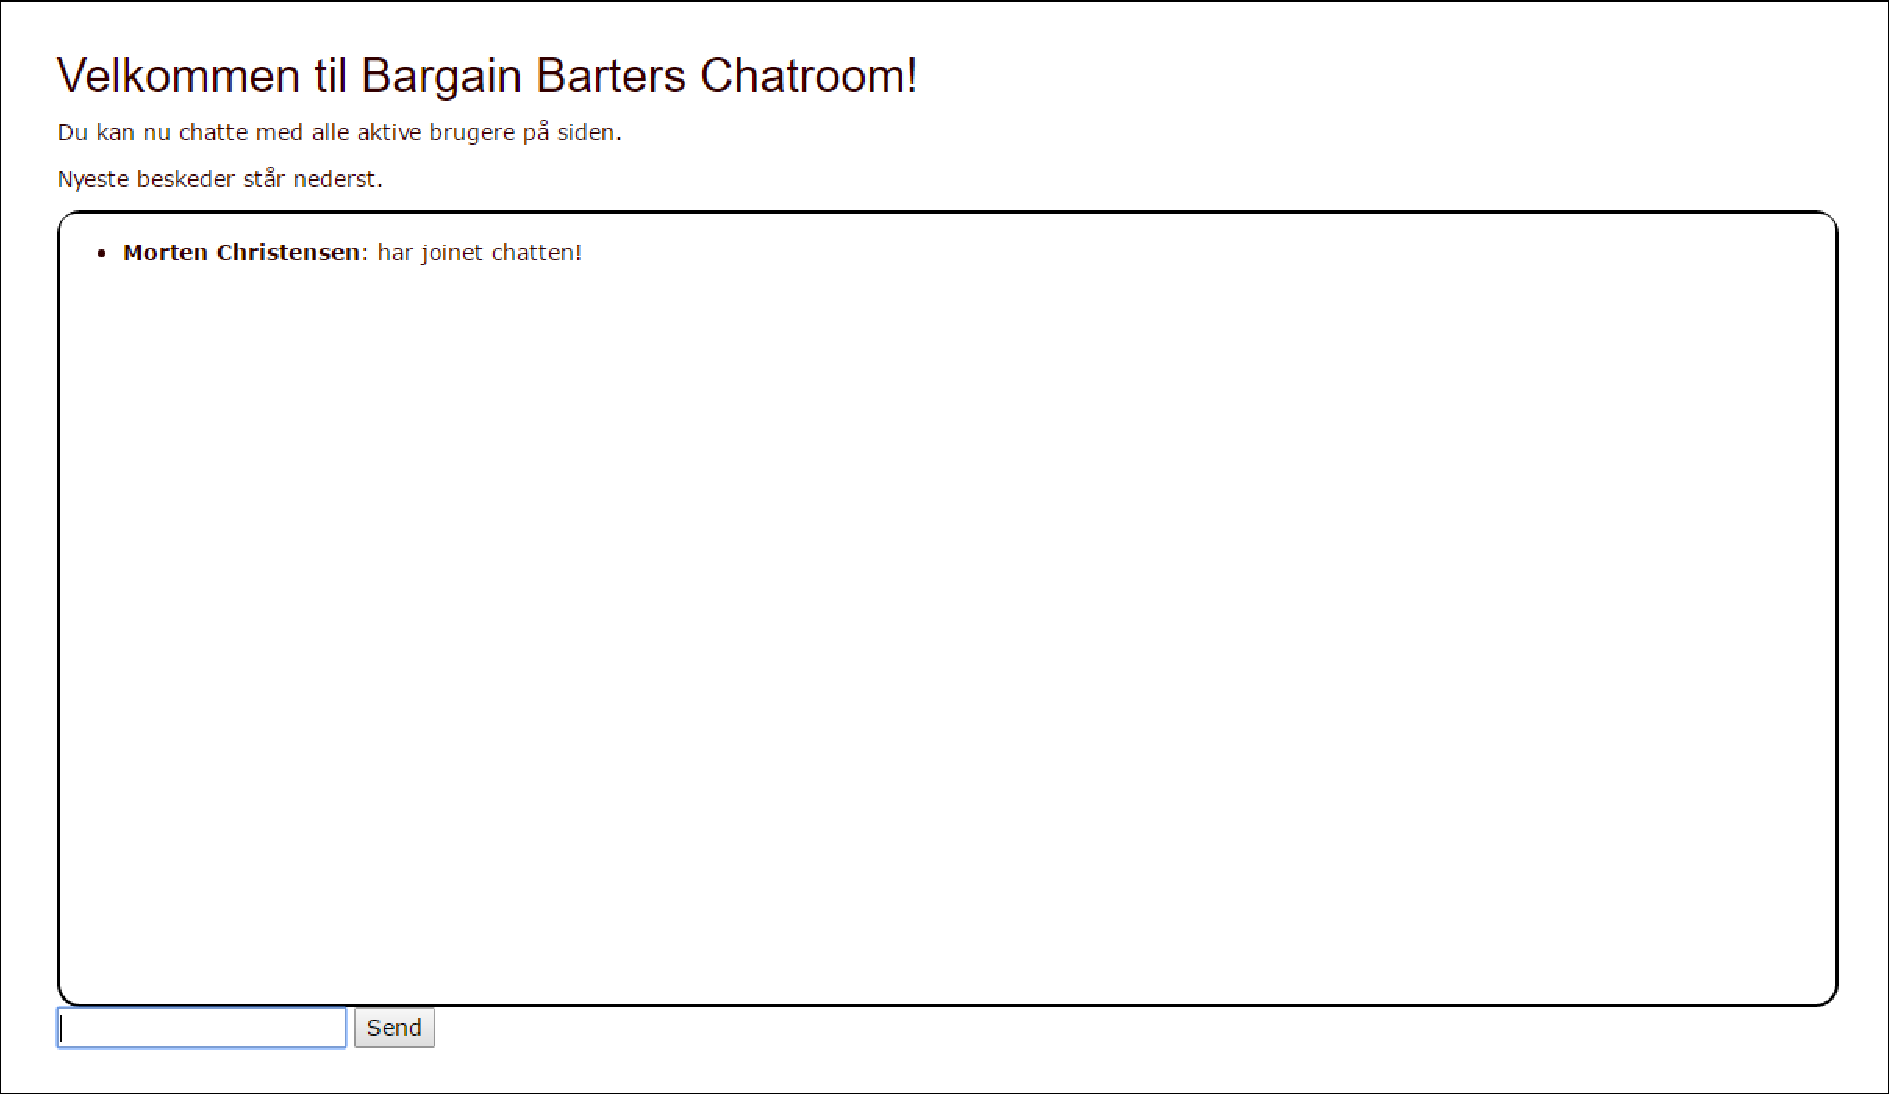
\includegraphics
	[width=165mm]{figures/chatroom.pdf}
	\caption{Screenshot af det færdige chatroom. }
	\label{fig:chatroom}
\end{figure}

På figur \ref{fig:chatroom} ses hvordan chatroomet ser ud på BargainBarter, som det fremvises når man første gang tilgår rummet. 

